\begin{enumerate}[label=\thesubsection.\arabic*.,ref=\thesubsection.\theenumi]
\item
	Using 
	\figref{fig:tri_sin_inc},
%Fig. \ref{trig_id_sin_theta}, 
show that 
	%
\begin{equation}
\label{trig_id_sin_theta_eq}
\sin  \theta_1 = \sin \brak{\theta_1 + \theta_2}\cos \theta_2 - \cos\brak{\theta_1+\theta_2}\sin\theta_2
\end{equation}	
	%
\iffalse
\begin{figure}[!ht]
	\begin{center}
		
		%\includegraphics[width=0.6\columnwidth]{figs/trig_id_sin_theta}
		%\vspace*{-10cm}
		{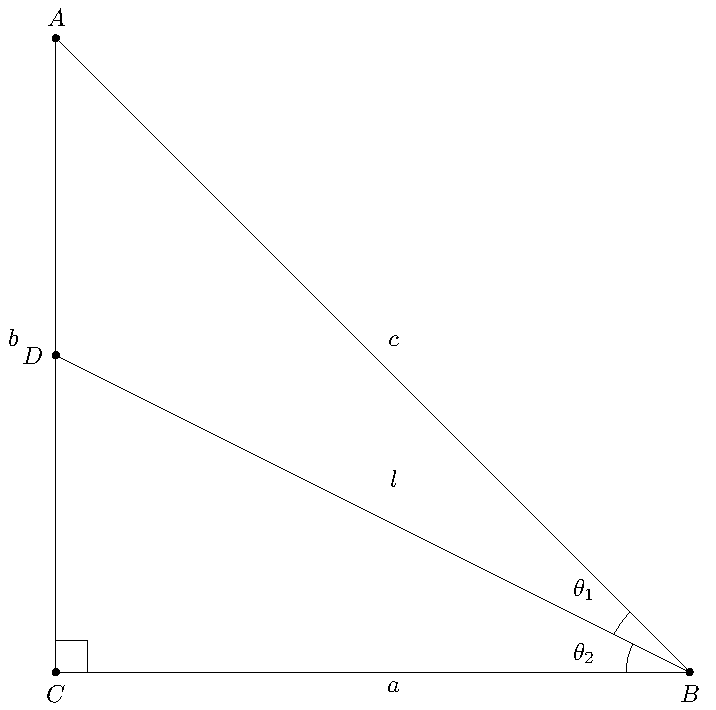
\includegraphics[width=0.6\columnwidth]{figs/trig_id/sincos/tri_sin_inc.pdf}}
	\end{center}
	\caption{$\sin \brak{\theta_1+\theta_2} = \sin\theta_1\cos\theta_2 + \cos\theta_1\sin\theta_2$}
	\label{trig_id_sin_theta}	
\end{figure}
\fi
%

\solution The following equations can be obtained from the figure using the forumula for the area of a triangle
%
\begin{align}
ar \brak{\Delta ABC} &= \frac{1}{2}ac \sin\brak{\theta_1 + \theta_2} \\
&= ar \brak{\Delta BDC} + ar \brak{\Delta ADB} \\
&= \frac{1}{2}cl \sin{\theta_1} + \frac{1}{2}al \sin{\theta_2} \\ 
&= \frac{1}{2}ac \sin{\theta_1} \sec \theta_2 + \frac{1}{2}a^2 \tan{\theta_2} 
\end{align}
$\brak{\because
	l = a \sec \theta_2}$.  From the above,
\begin{align}
\sin\brak{\theta_1 + \theta_2} &=  \sin{\theta_1} \sec \theta_2 + \frac{a}{c} \tan{\theta_2} \\
	&=  \sin{\theta_1} \sec \theta_2 
+ \cos\brak{\theta_1 + \theta_2} \tan{\theta_2} 
\end{align}
Multiplying both sides by $\cos \theta_2$,
\begin{align}
\sin\brak{\theta_1 + \theta_2}\cos{\theta_2} =  \sin{\theta_1}  
+ \cos\brak{\theta_1 + \theta_2} \sin\theta_2  
\end{align}
%
resulting in
\eqref{trig_id_sin_theta_eq}.
\item
	Prove the following identities 
	%
	\begin{enumerate}
\item 
\begin{equation}
		\label{trig_id_sin_diff}
\sin\brak{\alpha - \beta} = \sin \alpha \cos \beta - \cos \alpha \sin \beta.
\end{equation}
\item 
\begin{equation}
\cos\brak{\alpha + \beta} = \cos \alpha \cos \beta - \sin \alpha \sin \beta.
		\label{trig_id_cos_diff}
\end{equation}

	\end{enumerate}
	%

\solution In \eqref{trig_id_sin_theta_eq}, let
%
\begin{equation}
\begin{split}
\theta_1 + \theta_2 &= \alpha \\
\theta_2 &=  \beta
\end{split}
\end{equation}
%
This gives \eqref{trig_id_sin_diff}.  In \eqref{trig_id_sin_diff}, replace $\alpha$ by 
%
$90{\degree} - \alpha$.  This results in
%
\begin{align}
\sin\brak{90{\degree} - \alpha - \beta}
	&=
\sin \brak{90{\degree} -\alpha} \cos \beta - \cos \brak{90{\degree} -\alpha} \sin \beta \\
	\implies \cos\brak{\alpha + \beta} &= \cos \alpha \cos \beta - \sin \alpha \sin \beta
\end{align}
% 
\item
	Using \eqref{trig_id_sin_theta_eq} and \eqref{trig_id_cos_diff}, show that
\begin{align}
\label{trig_id_sin_sum}
\sin\brak{\theta_1 + \theta_2} &= \sin\theta_1  \cos\theta_2 + \cos\theta_1\sin\theta_2
\\
\cos\brak{\theta_1 - \theta_2} &= \cos\theta_1  \cos\theta_2  \sin\theta_1\sin\theta_2
\label{trig_id_cos_sum}
\end{align}

%
\solution From \eqref{trig_id_sin_theta_eq},
%
\begin{align}
 \sin \brak{\theta_1 + \theta_2}\cos \theta_2 =\sin  \theta_1 +\cos\brak{\theta_1+\theta_2}\sin\theta_2 
\end{align}
%
Using \eqref{trig_id_cos_diff} in the above,
%
\begin{align}
\sin \brak{\theta_1 + \theta_2}\cos \theta_2 
=\sin  \theta_1 +\brak{\cos \theta_1\cos\theta_2 
	- \sin \theta_1\sin\theta_2}\sin\theta_2 
\end{align}
%
which can be expressed as
%
\begin{align}
\sin \brak{\theta_1 + \theta_2}\cos \theta_2 
=\sin  \theta_1 
+\cos \theta_1\cos\theta_2 \sin\theta_2 
		- \sin \theta_1\sin^2\theta_2
\end{align}
%
Since
%
\begin{equation}
\sin^2\theta_2 = 1- \cos^2\theta_2, 
\end{equation}
%
we obtain
%
\begin{align}
\sin \brak{\theta_1 + \theta_2}\cos \theta_2 
=\cos \theta_1\cos\theta_2 \sin\theta_2 
+ \sin \theta_1\cos^2\theta_2
\end{align}
%
resulting in
%
\begin{equation}
\sin \brak{\theta_1 + \theta_2}
=\cos \theta_1 \sin\theta_2 
+ \sin \theta_1\cos\theta_2
\end{equation}
%
after factoring out $\cos \theta_2$.  Using a similar approach, \eqref{trig_id_cos_sum} can also be proved.
\item Show that 
\begin{align}
\label{eq:trig_id_sum_diff1}
\sin \theta_1 + \sin \theta_2 &= 2\sin\brak{\frac{\theta_1+\theta_2}{2}}\cos\brak{\frac{\theta_1-\theta_2}{2}}
\\
\label{eq:trig_id_sum_diff2}
\cos \theta_1 + \cos \theta_2 &= 2\cos\brak{\frac{\theta_1+\theta_2}{2}}\cos\brak{\frac{\theta_1-\theta_2}{2}}
\\
\label{eq:trig_id_sum_diff3}
\sin \theta_1 - \sin \theta_2 &= 2\sin\brak{\frac{\theta_1-\theta_2}{2}}\cos\brak{\frac{\theta_1+\theta_2}{2}}
\\
\label{eq:trig_id_sum_diff4}
\cos \theta_1 - \cos \theta_2 &= 2\sin\brak{\frac{\theta_1+\theta_2}{2}}\cos\brak{\frac{\theta_2-\theta_1}{2}}
\end{align}
%
\\
\solution Let 
%
\begin{align}
\label{eq:trig_id_ang_sum_diff}
\begin{split}
\theta_1 = \alpha + \beta
\\
\theta_2 = \alpha - \beta
\end{split}
\end{align}
%
From \eqref{trig_id_sin_sum},
%
\begin{align}
\sin \theta_1 + \sin \theta_2  &= \sin \brak{\alpha + \beta} + \sin \brak{\alpha - \beta}
\\
&= \sin \alpha \cos \beta + \cos \alpha \sin \beta 
+\sin \alpha \cos \beta - \cos \alpha \sin \beta
\\
&= 2 \sin \alpha \cos \beta
\end{align}
%
resulting in \eqref{eq:trig_id_sum_diff1}
%
\begin{align}
\because \alpha = \frac{\theta_1 +\theta_2}{2}
,\
\beta = \frac{\theta_1 -\theta_2}{2}
\end{align}
from \eqref{eq:trig_id_ang_sum_diff}.  Other identities may be proved similarly.
%
\item Show that 
  \begin{align}
\label{eq:trig-id-2A-sin}
	  \sin 2 \theta &= 2 \sin \theta \cos \theta
	  \\
	  \cos 2 \theta &= 1 - 2 \sin^2 \theta 
	  =  2 \cos^2 \theta -1
	  \\
	  &= \cos^2 \theta -\sin^2 \theta 
\label{eq:trig-id-2A-cos}
  \end{align}
\end{enumerate}
